\documentclass[autodetect-engine,dvipdfmx-if-dvi,ja=standard,b5paper,10.5pt,twoside,openany,layout=v2]{bxjsbook}

\newcommand{\stypath}{./sty}
\newcommand{\articlepath}{./articles}
\newcommand{\assetspath}{./assets}

\newcommand{\chikuwaitasset}{\assetspath/sample-chikuwa_ITasset/gray}
\newcommand{\haibaraasset}{\assetspath/sample-haibaraasset}

\usepackage{\stypath/localst17}
\usepackage{\stypath/mymintedsetting}

\usepackage{lipsum}
\usepackage{layout}

%keisuke495500
\usepackage{caption}

%Takuzoo3868
%\usepackage{dirtree}
\usepackage{here}
\usepackage{fontawesome}
\usepackage{tcolorbox}

%Jumpaku
\usepackage{pxrubrica}
\usepackage{hyperref}
\usepackage{pxjahyper}
\usepackage{comment}
\usepackage{verbatim}

%materialofmouse
%\usepackage{siunitx}

\usepackage{amsmath}
\usepackage{graphicx}

%HSAU_Dosei
\usepackage{ulem}

\title{学生部同人誌2020sandbox}
\author{はいばら \and ちくうぇいと }

\date{}

\begin{document}
\frontmatter
\maketitle
\begin{myintroduce}{\haibaraasset/icon.jpg}{はいばら @haibara}
  美味しいご飯とソフトウェアとハードウェアがすきです.\\
  LOCAL学生部の部長をしています.
\end{myintroduce}
\begin{myintroduce}{\chikuwaitasset/icon.jpg}{chikuwait}
 ちくわさんです
\end{myintroduce}


\chapter{はじめに}
\addtolength{\oddsidemargin}{10pt}
\addtolength{\evensidemargin}{-10pt}
%\addtolength{\textwidth}{-14pt}
LOCALがくせーぶの紹介とかなんか.部長!お願いしますよ! by さわだ


\tableofcontents
\mainmatter
%\addtolength{\oddsidemargin}{-20pt}
%\addtolength{\evensidemargin}{18pt}

\chapterauthor{はいばら}
\chapter{ESP-WROOM-02で作る \\自走式Webサーバー入門}
\section{はじめに}
自宅サーバー,憧れますよね.そんな自宅サーバーをお手頃な価格で自作してしまいましょう.せっかくなのでモーターとタイヤをつけてしまいましょう.そうです,自走式Webサーバーです.この章ではWi-Fiを扱うことのできるマイコン ESP-WROOM-02を用いた自走式Webサーバーを作成します(図 \ref{fig:webserver}).
\footnote{本章に記載されたプログラム,回路図,その他工作物を参考にして製作した場合に生じた事故等について一切の責任を負いかねます.}
\subsection{ESP-WROOM-02とは}
ESP-WROOM-02は,上海の企業Espressif Systems のESP8266EXチップを搭載したWi-Fiモジュールです.いわゆる「技適」を取得しているため,日本国内で法的に安心して使えます.arduino言語で開発できることに加え,おおよそ600円で購入できる手軽さが魅力です.
\footnote{ESP-WROOM-02の開発環境の構築方法については, ESP8266 Arduino Coreの公式ドキュメント(\url{https://arduino-esp8266.readthedocs.io/en/latest/})や,僕のブログ(\url{https://haibara-works.hatenablog.com})の『ESP-WROOM-02を導入する』を参照してください.(ページ数の都合から本章ではその説明は割愛します)}

\begin{figure}[htbp]
    \centering
    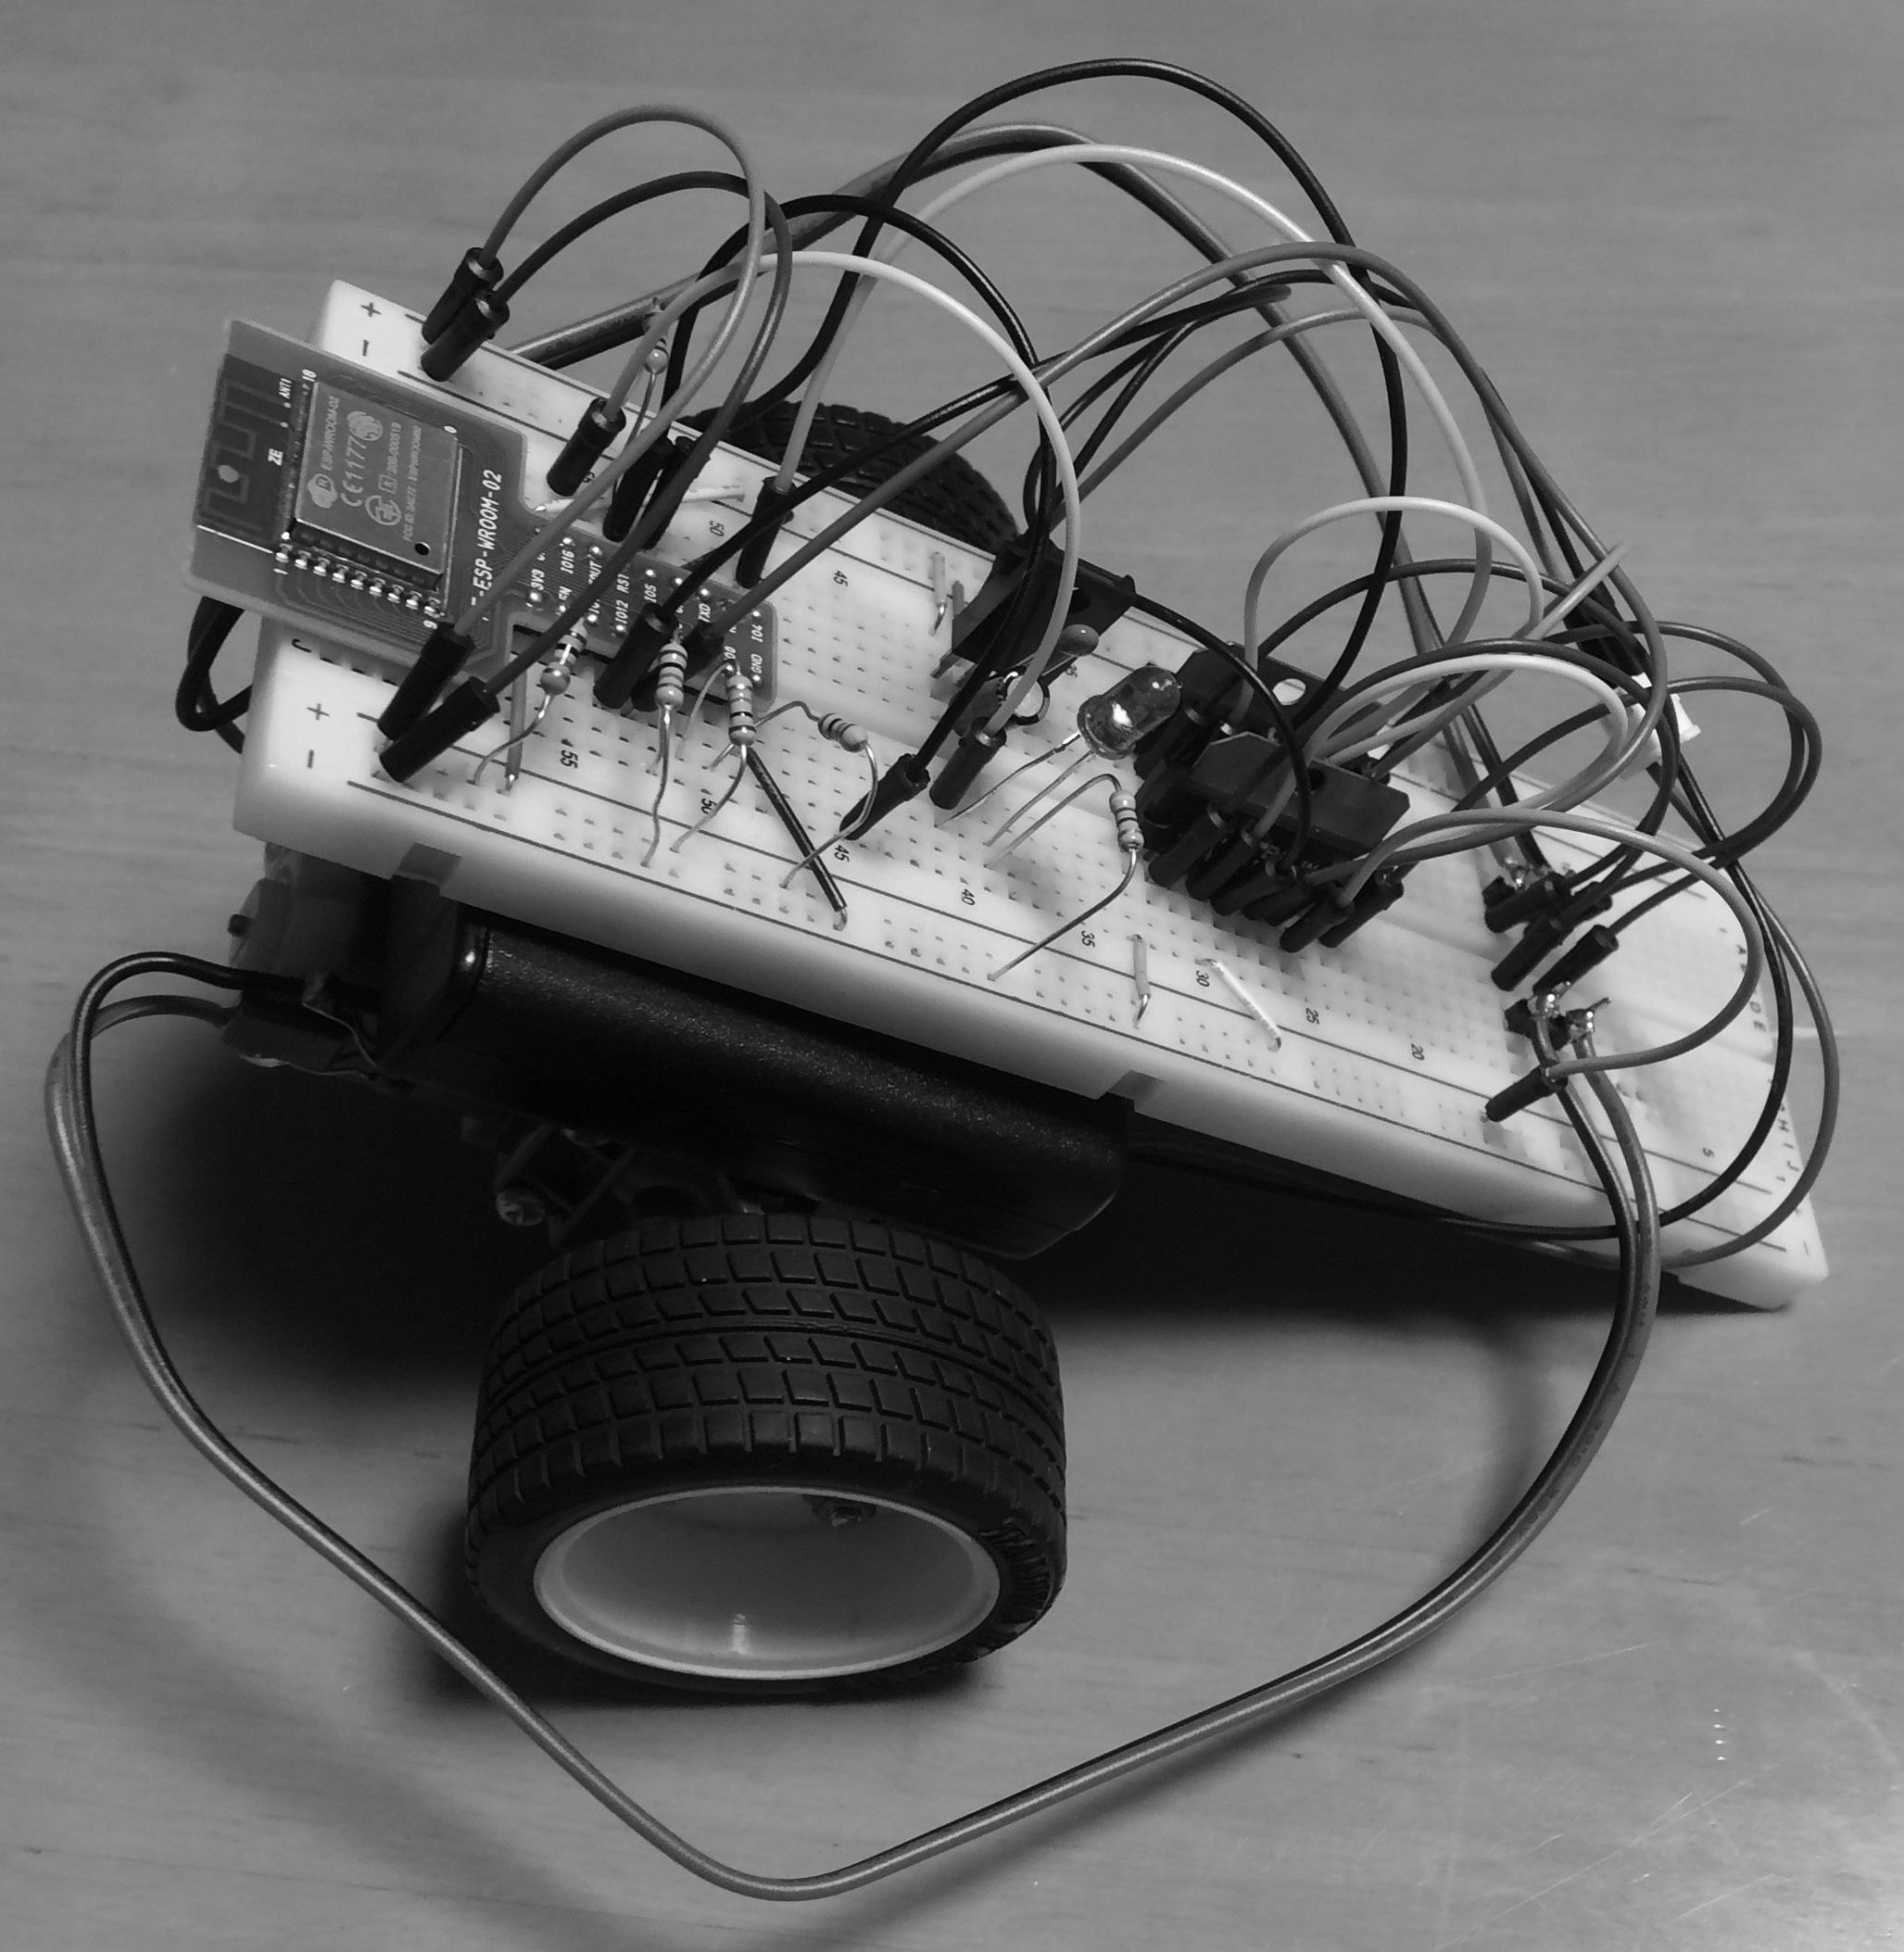
\includegraphics[width=50mm]{./assets/sample-haibaraasset/webserver.jpg}
    \caption{自走式Webサーバーの実装例}
    \label{fig:webserver}
\end{figure}

\subsection{ハードウェアの準備}
表\ref{buhin}に今回作る自走式Webサーバーに必要な部品を示します.
\begin{table}[htb]
\centering
\caption{使うもの}
\begin{tabular}{|l|l|} \hline
部品 & 用途 \\ \hline \hline
ESP-WROOM-02 & ESP本体  \\ \hline
FT-232RQ & USBシリアル変換モジュール  \\ \hline
抵抗(10 k$\Omega$) & プルアップ・プルダウン用  \\ \hline
抵抗(470 k$\Omega$) & LEDの保護抵抗 \\ \hline
LED & パイロットランプ  \\ \hline
TA48033S & 電源レギュレータ(3.3 V) \\ \hline
コンデンサ(0.33 $\mu$F) & 電源用パスコン  \\ \hline
コンデンサ(33 $\mu$F) & 電源用パスコン  \\ \hline
TA7291P & モータードライバ \\ \hline
ダブルギヤボックス(左右独立4速タイプ) & タミヤのギヤボックス  \\ \hline
ブレッドボード & テスト用 \\ \hline
ジャンパ線 & テスト用 \\ \hline
\end{tabular}
\label{buhin}
\end{table}

\section{ラジコンとしての動作}
\subsection{モータードライバの利用}
    モーターの制御にはモータードライバIC TA7291Pを使用します.このICはArduinoの入門記事などでよく登場する,とても扱いやすいICです.制御方法も簡単で,2つの入力端子をマイコンのGPOに接続し,2つの出力をモーターのそれぞれの端子に接続して使います.以下にTA7291Pの真理値表を示します.
\footnote{表中のZはハイインピーダンス(LともHとも定まらない状態)を表します}
\footnote{正転・逆転はモーターの端子とOUT1・OUT2との接続の仕方によっては逆になります.}

\begin{table}[H]
\centering
\caption{TA7291Pの動作}
\begin{tabular}{|l|l|l|l|l|} \hline
IN1 & IN2 & OUT1 & OUT2 & 用途 \\ \hline \hline
L & L & Z & Z & オープン \\ \hline
L & H & L & H & 正転 \\ \hline
H & L & H & L & 逆転 \\ \hline
H & H & L & L & ブレーキ \\ \hline
\end{tabular}
\label{buhin}
\end{table}

また,真理値表の正転・逆転の際のHをPWM出力にすれば,PWM波形のデューティ比に応じたスピードでモーターを制御することができます.
つまり,以下のコードがTA7291Pを用いたモーター制御の基本になります.
\begin{minted}[frame=lines,framesep=2mm,baselinestretch=1.2,fontsize=\footnotesize,linenos,breaklines]{c}
analogWrite(motorPin1, pwmValue);
digitalWrite(motorPin2, LOW);
\end{minted}
これを左右のモーターそれぞれに適応させ,前進・後進・右旋回・左旋回をさせます.

\subsection{Webからの操作}
Webページからモーターを制御するために,URLクエリ文字列を利用します.URLクエリ文字列とはURLに付帯する引数のようなもので,たとえば\url{192.168.4.10/?val=abc}というURLであれば``valという引数の値はabcである"と解釈されます.また\url{192.168.4.10/?val1=abc&val2=123}というように\&で結ぶことで複数の引数を付帯させることもできます.ESPでは\tt{ESP8266WebServer.h}\rm{}でURLクエリ文字列の取得に関するかいくつかの関数が定義されています.次の関数はそれらの使用例です.
\begin{minted}[frame=lines,framesep=2mm,baselinestretch=1.2,fontsize=\footnotesize,linenos,breaklines]{c}
/**  Show URI args */
void showUriArgs() {
  Serial.println("---URI args---");
  for (int i = 0; i < Server.args(); i++) { //Server.args(): クエリ文字列の引数の個数を取得
    Serial.printf("%s: %s \n", Server.argName(i).c_str(), Server.arg(i).c_str()); 
    //Server.argName(num): クエリ文字列のnum番目の引数名を取得
    //Server.arg(num); クエリ文字列のnum番目の引数の値を取得
  }
}
\end{minted}
ESPに\url{192.168.4.10/?val1=abc&val2=123}というURLへリクエストがあった際にこの関数が実行されると,シリアルコンソールには
\tt{

---URL args---

val1: abc

val2: 123

}\rm{}
\noindent
と表示されるはずです.
また,\tt{Server.arg("val")}\rm{}というように\tt{Server.arg()}\rm{}にクエリ文字列の引数名を渡すと,その引数の値を取得できます.
今回のコードではWebサーバーの進行方向をmotorModeで,モーターの回転速度をmotorValでそれぞれ指定することにします.
ボタンとスライダーでこれら2つの値を指定する簡易的な操作画面をHTMLとjsで示しました.(図 \ref{fig:html})

\begin{figure}[htbp]
    \centering
    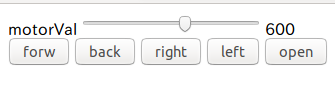
\includegraphics[width=50mm]{./assets/sample-haibaraasset/motorCtr.png}
    \caption{自走式Webサーバーの操作画面}
    \label{fig:html}
\end{figure}

\begin{minted}[frame=lines,framesep=2mm,baselinestretch=1.2,fontsize=\footnotesize,linenos,breaklines]{c}
enum { M1_l = 4, M1_r = 5, M2_l = 12, M2_r = 13, Pilot = 16, //モーターを接続するピン及びパイロットランプを接続するピンの定義
       Stop, Open, Forw, Back, Right, Left }; //motorModeの値となる定数

typedef struct {
  int _mode; //Webサーバーの進行方向を格納
  int val; //モーターの回転速度を格納
} motor_T;
motor_T motor;

/**************************************************
  モーター制御に関する関数群
 **************************************************/
/**  左右2つのモーターに接続されるピンを初期化 */
void motorSetup(const int m1_l, const int m1_r, const int m2_l, const int m2_r) {
  pinMode(m1_l, OUTPUT);
  pinMode(m1_r, OUTPUT);
  pinMode(m2_l, OUTPUT);
  pinMode(m2_r, OUTPUT);

  digitalWrite(m1_l, LOW);
  digitalWrite(m1_r, LOW);
  digitalWrite(m2_l, LOW);
  digitalWrite(m2_r, LOW);

  analogWriteFreq(5);
}

/**  モーターをPWM制御する関数 */
void motorDrive(int16_t pwmVal, const int m_l, const int m_r) {
  pwmVal = constrain(pwmVal, -1024, 1024);

  if (pwmVal >= 0) {
    analogWrite(m_l, pwmVal);
    digitalWrite(m_r, LOW);
  } else {
    pwmVal = abs(pwmVal);

    digitalWrite(m_l, LOW);
    analogWrite(m_r, pwmVal);
  }
}

/**  stop */
void stopMotor() {
  digitalWrite(M1_l, LOW);
  digitalWrite(M1_r, LOW);
  digitalWrite(M2_l, LOW);
  digitalWrite(M2_r, LOW);
}

/**  前進 */
void goForward(int16_t velocity) {
  motorDrive(velocity, M1_l, M1_r);
  motorDrive(velocity, M2_l, M2_r);
}

/**  後進 */
void goBack(int16_t velocity) {
  motorDrive(-velocity, M1_l, M1_r);
  motorDrive(-velocity, M2_l, M2_r);
}

/**  右旋回 */
void turnRight(int16_t velocity) {
  motorDrive(velocity, M1_l, M1_r);
  motorDrive(-velocity, M2_l, M2_r);
}

/**  右旋回 */
void turnLeft(int16_t velocity) {
  motorDrive(-velocity, M1_l, M1_r);
  motorDrive(velocity, M2_l, M2_r);
}
\end{minted}

\section{Webサーバーとしての動作}
最低限のWebサーバーとして,クライアントがHTTP GETでページを取得できること,不揮発性メモリにファイルを保存できること,不揮発性メモリ内のファイルを作成・編集・削除できるようにすること,の3つの機能を実装しました.
\subsection{SPIFFSの利用}
ESPではSPIFFSというファイルシステムを使うことが出来ます.これはESPの不揮発性メモリの一部をストレージとして使えるようにするもので,プログラム中からC言語の\tt{fopen()}\rm{} と同じ要領でメモリにアクセス出来ます.この機能を用いてESPにファイルを保存します.
また,ArduinoIDEにSPIFFSプラグイン(\url{https://github.com/esp8266/arduino-esp8266fs-plugin})をインストールすると,ArduinoIDEからESPのSPIFFSにファイルをアップロードすることができます.
ESP8266 Arduino Coreの公式exampleの中にFSBrowserというスケッチが,まさにSPIFFSを用いたWebサーバーの実装になっています(\url{https://github.com/esp8266/Arduino/tree/master/libraries/ESP8266WebServer/examples/FSBrowser}).
このスケッチにある関数\tt{String formatBytes(size\_t bytes)}\rm{}・\tt{bool handleFileRead(String path)}\rm{}・\tt{void handleFileUpload()}\rm{}・\tt{void handleFileDelete()}\rm{}・\tt{void  handleFileCreate()}\rm{}・\tt{void  handleFileList()}\rm{}を利用します.
また,FSBrowser.inoと同じディレクトリの\tt{/data}\rm{}内にはいくつかのjsファイルやhtmlファイルが保存されています.その中にはSPIFFSに保存されているファイルの編集・削除,新規ファイルのアップロードを行うことのできるWebGUIとして働くものや,現在のヒープメモリやGPIOの電位などをグラフで提供するものが含まれています.(図 \ref{fig:fsb})今回はこれらの\tt{/data}\rm{}内のファイルを使用して,SPIFFS管理のためのWebGUIとします.

\begin{figure}[htbp]
    \centering
    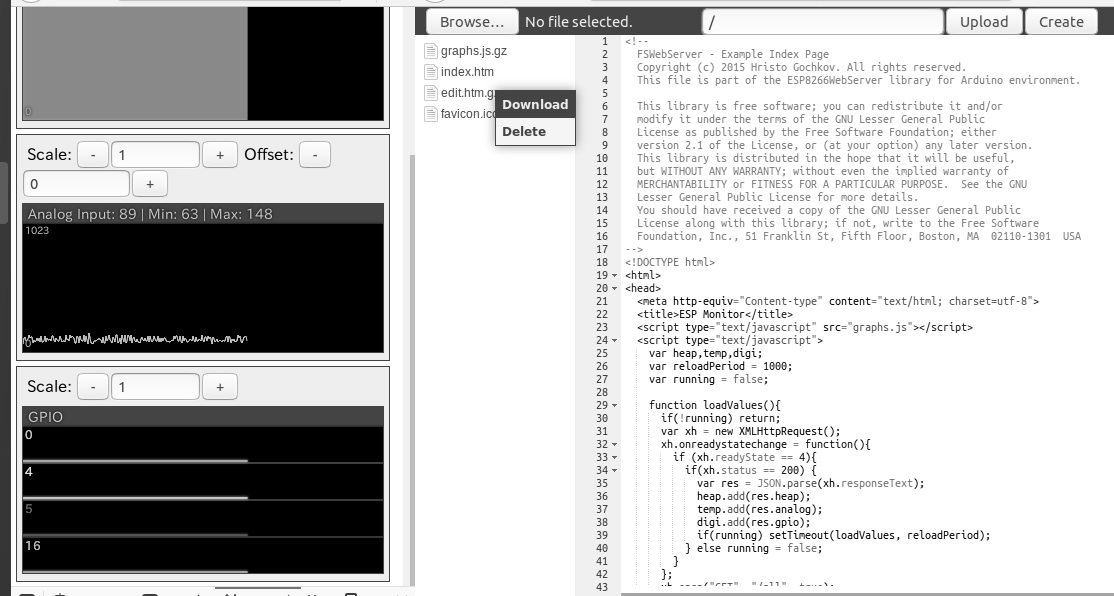
\includegraphics[width=50mm]{./assets/sample-haibaraasset/FSBrowser.png}
    \caption{FSBrowserのWebGUI}
    \label{fig:fsb}
\end{figure}

\subsection{Webページの表示}
\tt{ESP8266WebSerber.h}\rm{}を用いて,クライアントからのHTTPリクエストを処理する際には,\tt{Server.on(path, handlerFunction);}\rm{}と記述することで,``\tt{path}\rm{}がリクエストされたら\tt{handlerFunction}\rm{}を実行する"ということができます.しかし,この方法では処理できる\tt{path}\rm{}の種類がコーディングの時点で固定されてしまいます.今回のようにSPIFFSを用いて,動的にファイルが変わり得る場合はどのように対処すればいいでしょうか.1つの方法は\tt{Server.on(path, handlerFunction)}\rm{}ではなく\tt{Server,onNotFound(handlerFunction)}\rm{}を用いることです.これはクライアントにリクエストされた\tt{path}\rm{}がどの\tt{Server.on}\rm{}でも指定されていない場合に,\tt{handlerFunction}\rm{}を呼び出すという関数で,その名の通り404 Not Foundを返すために使われます.しかし\tt{Server.on}\rm{}を記述しなければ任意の\tt{path}\rm{}がリクエストされたときに必ず\tt{handlerFunction}\rm{}が呼ばれます.この\tt{handlerFunction}\rm{}内で``リクエストされた\tt{path}\rm{}はSPIFFSに存在するか"を判断し,存在すればその\tt{path}\rm{}ごとの処理をし,存在しなければ404 Not Foundをクライアントに送信するという処理を行うことで,SPIFFS内の動的ファイルの変化に対応できます.

\begin{minted}[frame=lines,framesep=2mm,baselinestretch=1.2,fontsize=\footnotesize,linenos,breaklines]{c}
#include <ESP8266WiFi.h>
#include <WiFiClient.h>
#include <ESP8266mDNS.h>
#include <ESP8266WebServer.h>
#include <ESP8266HTTPUpdateServer.h>
#include <FS.h>
#include "config.h"

const char* host = "esp8266fs";
ESP8266WebServer Server(80);      //80番ポートを使用

/**************************************************
  Webサーバーに関する関数群
 **************************************************/
/**  Show URI args */
void showUriArgs() {
  Serial.printf("\n---URI args---\n");
  for (int i = 0; i < Server.args(); i++) {
    Serial.printf("%s: %s \n", Server.argName(i).c_str(), Server.arg(i).c_str());
  }
}

/**  ファイルの拡張子を調べてMIMEタイプを返す関数 */
String getContentType(String filename) {
  if (Server.hasArg("download")) return "application/octet-stream";
  else if (filename.endsWith(".htm")) return "text/html";
  else if (filename.endsWith(".html")) return "text/html";
  else if (filename.endsWith(".css")) return "text/css";
  else if (filename.endsWith(".js")) return "application/javascript";
  else if (filename.endsWith(".png")) return "image/png";
  else if (filename.endsWith(".gif")) return "image/gif";
  else if (filename.endsWith(".jpg")) return "image/jpeg";
  else if (filename.endsWith(".ico")) return "image/x-icon";
  else if (filename.endsWith(".xml")) return "text/xml";
  else if (filename.endsWith(".pdf")) return "application/x-pdf";
  else if (filename.endsWith(".zip")) return "application/x-zip";
  else if (filename.endsWith(".gz")) return "application/x-gzip";
  else return "text/plain";
}

/**  指定されたパスのファイルをクライアントに送信 */
void handleSendRes(void) {
  showUriArgs();
  String path = Server.uri();

  if (path.equals("/motor.html")) {
    motor._mode = Open;
    if (Server.arg("motorMode").equals("forw")) {
      motor._mode = Forw;
    } else if (Server.arg("motorMode").equals("back")) {
      motor._mode = Back;
    } else if (Server.arg("motorMode").equals("right")) {
      motor._mode = Right;
    } else if (Server.arg("motorMode").equals("left")) {
      motor._mode = Left;
    }
    motor.val = atoi(Server.arg("motorVal").c_str());
  }

  Serial.println("");
  Serial.println("[handleSendRes]: trying to read " + path);

  if (path.endsWith("/")) path += "index.html";

  String contentType = getContentType(path);

  if (SPIFFS.exists(path)) {
    Serial.println("[handleSendRes]: sending " + path);
    File file = SPIFFS.open(path, "r");
    Server.streamFile(file, contentType);
    file.close();
    Serial.println("[handleSendRes]: sent " + path);
  } else {
    Serial.println("[handleSendRes]: 404 not found");
    Server.send (404, "text/plain", "ESP: 404 not found");
  }
}

/**  settings */
void setup() {
  motor._mode = Open;
  motor.val = 0;

  Serial.begin(74880);

  pinMode(Pilot, OUTPUT);
  digitalWrite(Pilot, HIGH);

  motorSetup(M1_l, M1_r, M2_l, M2_r);

  WiFi.mode(WIFI_STA);
  WiFi.begin(ssid, pass);
  delay(100);

  Serial.println("");

  while (WiFi.status() != WL_CONNECTED) {
    delay(500);
    digitalWrite(Pilot, !digitalRead(Pilot));
    Serial.print(".");
  }
  digitalWrite(Pilot, HIGH);

  Serial.println("");
  Serial.print("Connected to ");
  Serial.println(ssid);
  Serial.print("IP address: ");
  Serial.println(WiFi.localIP());
  MDNS.begin(host);

  SPIFFS.begin();
  {
    Dir dir = SPIFFS.openDir("/");
    while (dir.next()) {
      String fileName = dir.fileName();
      size_t fileSize = dir.fileSize();
      Serial.printf("FS File: %s, size: %s\n", fileName.c_str(), formatBytes(fileSize).c_str());
    }
    Serial.printf("\n");
  }

  //  ウェブサーバの設定
  Server.on("/list", HTTP_GET, handleFileList);
  Server.on("/edit", HTTP_GET, []() {
    if (!handleFileRead("/edit.htm")) {
      Server.send(404, "text/plain", "FileNotFound");
    }
  });
  Server.on("/edit", HTTP_PUT, handleFileCreate);
  Server.on("/edit", HTTP_DELETE, handleFileDelete);
  Server.on("/edit", HTTP_POST, []() {
    Server.send(200, "text/plain", "");
  }, handleFileUpload); 
  Server.on("/all", HTTP_GET, []() {
    String json = "{";
    json += "\"heap\":" + String(ESP.getFreeHeap());
    json += ", \"analog\":" + String(analogRead(A0));
    json += ", \"gpio\":" + String((uint32_t)(((GPI | GPO) & 0xFFFF) | ((GP16I & 0x01) << 16)));
    json += "}";
    Server.send(200, "text/json", json);
    json = String();
  });
  Server.onNotFound(handleSendRes);
  
  Server.begin();
}

/**  main loop */
void loop() {
  Server.handleClient();
  MDNS.update();

  switch (motor._mode) { //motor.modeの値によって進行方向を決定する
    case Forw:
      goForward(motor.val);
      break;
    case Back:
      goBack(motor.val);
      break;
    case Right:
      turnRight(motor.val);
      break;
    case Left:
      turnLeft(motor.val);
      break;
    case Open:
    default:
      stopMotor();
  }
}
\end{minted}

\section{おわりに}
ESP-WROOM-02を使って自走式Webサーバーを作成することができました.今後の課題として,websocketを用いたリアルタイム性の高い操作を実現したいです.
今回作成したソースコードは以下のレポジトリにあります.\url{https://github.com/w-haibara/Self-propelledWebServer}


\chapterauthor{ちくうぇいと}
\chapter{ちくわさんの記事}
\section{はじめに}
近年, コンテナ型仮想化の普及もあり仮想化技術という存在を様々な場面でよく聞くようになりました. しかし, コンテナ型仮想化技術以外の他の仮想化技術というのは中々個人で扱うような技術・ソフトウェアではないこともあり, あまり知られていないことが多かったりします. また, コンテナ型仮想化技術も便利で環境構築が魔法のようなすごい存在といった漠然とした解釈の人もきっと多いはずです. そこでこの章では, 各種仮想化技術の仕組みや特徴について触れながらふわっと仮想化技術について紹介します.

\section{仮想化技術とは}
仮想化技術にはいくつか種類がありますが, この章では計算機資源を抽象化してOSなどに見せるプラットフォーム仮想化のことを指します. 仮想化することで複数の計算機資源を単一に見せたり, 単一の計算機資源を複数に見せることができます. そしてプラットフォーム仮想化を支えるための技術としてシステム仮想機械(VM, Virtual Machine)と呼ばれる計算機資源をエミュレートするソフトウェアが存在します. 仮想機械の実装はハイパーバイザを始めとしていくつか存在します. 例えば仮想専用サーバ(VPS, Virtual Private Server)のようなサービスでは図2.1にように, 物理サーバ上に仮想化OSによって複数の仮想サーバに分割してユーザに各仮想サーバを提供しています.
\begin{figure}[htbp]
    \centering
    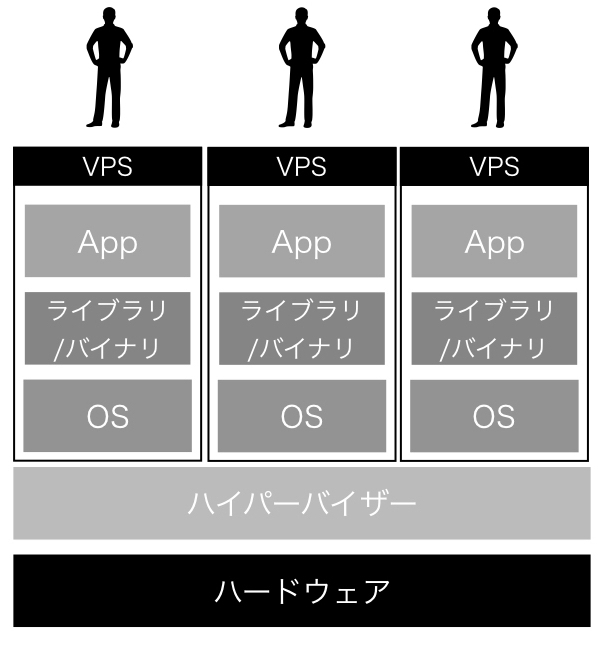
\includegraphics[width=80mm]{./assets/sample-chikuwa_ITasset/gray/vps.jpeg}
    \caption{VPSのイメージ}
    \label{fig:vps}
\end{figure}

\section{ハイパーバイザについて}
仮想化を実現するハイパーバイザにはベアメタル型(Type1),ホスト型(Type2)の2つに分類されます.

\section{ベアメタル型(Type1)}
ベアメタル型(Type1)は, ハードウェアの上で直接動作します. この方式ではホストOSと呼ばれるような土台になるOSが存在しないため,仮想マシンによる遅延や速度低下を防ぐことができます. そしてベアメタルハイパーバイザでは実装手法でもモノリシックカーネル型とマイクロカーネル型の2つに分類することができるほか, 仮想化のアプローチで完全仮想化と準仮想化に分類することができます.
\subsection{モノリシックカーネル型}
主にVMware ESX/ESXiなどで採用されている方式で, モノリシックという英語で「1枚岩」という意味の通り,図2.2のようにハイパーバイザの中にデバイスドライバが含まれています. ハイパーバイザがストレージをはじめ,ネットワークや入力デバイスといったハードウェアへのアクセスをすべてを処理します. この方法の利点はハイパーバイザとデバイスドライバが密接に連携するため,オーバーヘッドが少なく効率的であることです. しかしながら, ハイパーバイザの中にデバイスドライバが存在しているため,ハイパーバイザ層でデバイスドライバを用意する必要があります. そのため, ハードウェアのサポートがマイクロカーネル型と比較して少なく, 使用するハードウェアに制限がかかってしまう場合があります. また, デバイスドライバをハイパーバイザに直接組み込むため, バグや脆弱性はハイパーバイザ全体に広がってしまいます.
\begin{figure}[htbp]
    \centering
    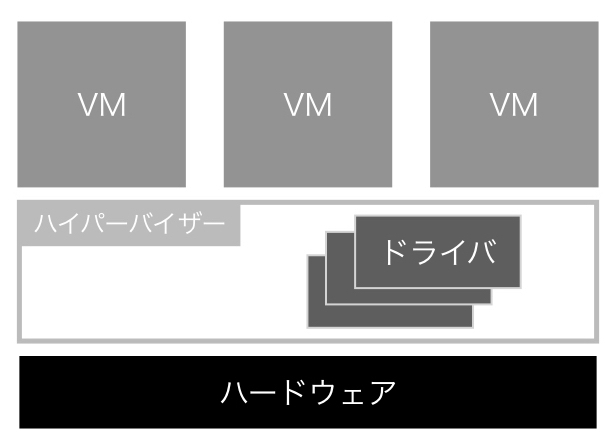
\includegraphics[width=80mm]{./assets/sample-chikuwa_ITasset/gray/monolithic.jpeg}
    \caption{モノリシックカーネル型ベアメタルハイパーバイザ}
    \label{fig:monolithic}
\end{figure}
\subsection{マイクロカーネル型}
主にXenやHyper-Vで採用されている方式で, 図2.3のようにハイパーバイザを管理する仮想マシンと管理OSを用意します. この管理OSはLinuxはWindows Serverなど汎用OSを使用します. また, 管理OSはXenではドメイン0, Hyper-Vでは親パーティションと呼ばれています. この方式では, 図2.4のようにデバイスドライバはハイパーバイザではなく, ハイパーバイザ上の仮想マシンとして動作している管理OSのデバイスドライバを使用します. 仮想マシンからハードウェアにアクセスする時はゲストOSから仮想デバイスのインターフェースを経由してハイパーバイザから管理OSに渡されます. そして管理OSのデバイスドライバからハードウェアにアクセスします.この方法は, 汎用OSのデバイスドライバを使用することで, モノリシックカーネル型に比べてハードウェアのサポートが多く, ハードウェアの対応が柔軟であるという利点があります. 例えば, Hyper-VならWindows用のデバイスドライバを使用することができます. しかしながら, ハードウェアにアクセスする際にハイパーバイザから管理OSを経由するため, モノリシックカーネル型よりも性能が低下してしまいがちであり, 管理用の汎用OSがクラッシュした場合全てのVMがクラッシュしてしまうといった欠点が存在します.
\begin{figure}[htbp]
    \centering
    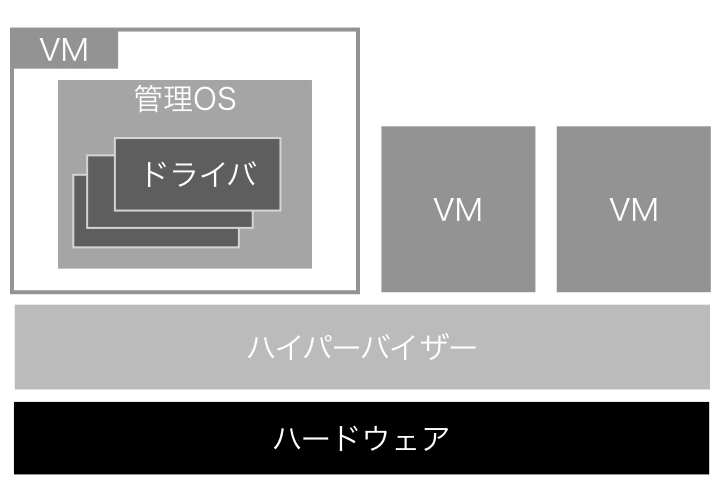
\includegraphics[width=80mm]{./assets/sample-chikuwa_ITasset/gray/microkernel.jpeg}
    \caption{マイクロカーネル型ベアメタルハイパーバイザ}
    \label{fig:microkernel}
\end{figure}
\begin{figure}[htbp]
    \centering
    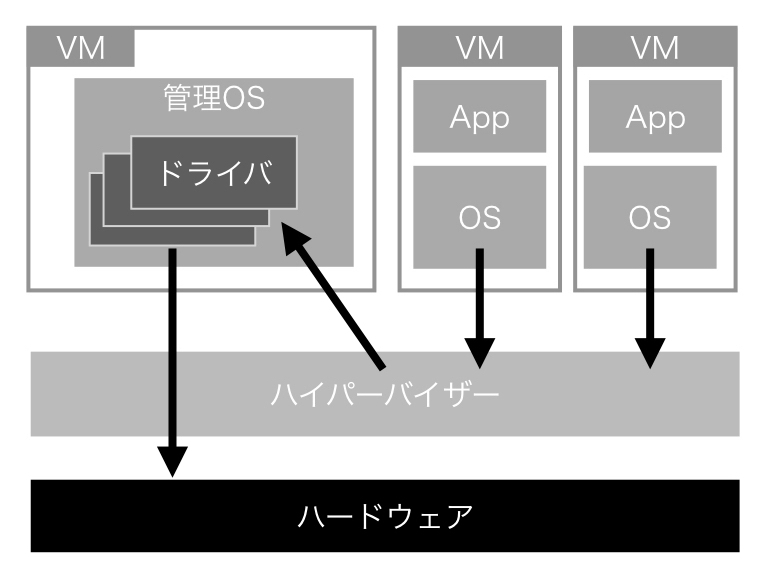
\includegraphics[width=80mm]{./assets/sample-chikuwa_ITasset/gray/microkernel_hardware.jpeg}
    \caption{マイクロカーネル型のハードウェアアクセス}
    \label{fig:microkernel_access}
\end{figure}

\subsection{完全仮想化}
完全仮想化方式のハイパーバイザでは, ハードウェアの挙動をすべてエミュレートします. そのため, 何も変更も加えていないそのままのホストOSを動かすことができます. 1960年代にIBMが「トラップアンドエミュレート」とよばれる方法で完全仮想化を実装しようとしました. この方法ではゲストOSが特権がない状態(Ring3)で実行させ, 特権(Ring0)が必要な命令を実行しようとすると失敗します. その際にハイパーバイザがその失敗をトラップして原因を確認してからその命令をエミュレートすることによってゲストOSの期待する結果を返すことができ, ゲストOSにRing0以外で実行されていることを気づかせないようにすることができます. しかしながら, この手法は古典的ですべてのアーキテクチャに適用できるわけではありませんでした. 特にx86プロセッサの場合, ユーザ権限で実行できるセンシティブ命令と呼ばれる計算機資源の構成などの依存している命令が存在しているため, 実装を難しくさせていました. そこで, 「バイナリトランスレーション」と呼ばれる新しい手法が使われるようになりました. この手法では, センシティブな命令以外の命令は直接CPUで実行し, センシティブな命令はハイパーバイザで実行前に動的に他の命令に置き換えられます.
\begin{figure}[htbp]
    \centering
    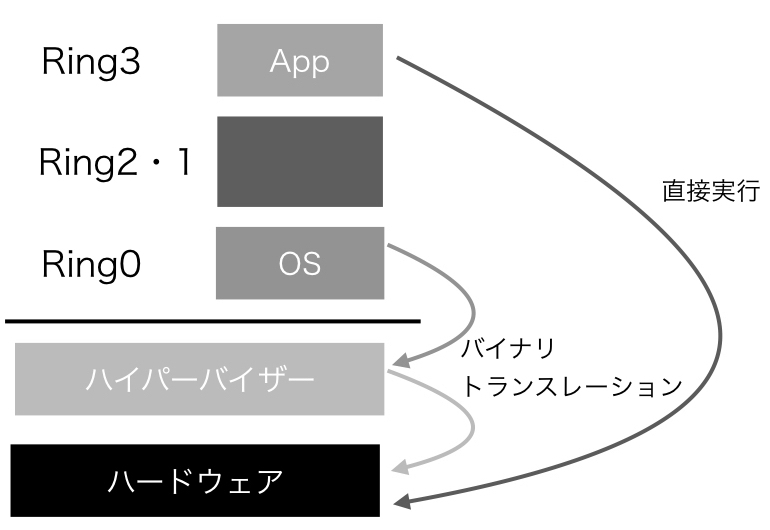
\includegraphics[width=80mm]{./assets/sample-chikuwa_ITasset/gray/binarytransration.jpeg}
    \caption{バイナリトランスレーション}
    \label{fig:binarytranslation}
\end{figure}
\subsection{準仮想化}
準仮想化方式のハイパーバイザでは, ハイパーバイザ上で実行するゲストOSに手を加え, 仮想環境を実現しています. この方式では, ゲストOSのカーネルが発行するハードウェアを制御するシステムコールに手を加えることでハイパーバイザと協調することで高速に動作させようとするものです. なおこのような手を加えられたシステムコールはハイパーバイザコールと呼ばれます. バイナリトランスレーションではセンシティブ命令を動的に変換していたため,性能が低下しやすい特徴がありましたが, 準仮想化では静的に変換を行い修正するため, 性能には影響はありません. しかしながら, ゲストOSに予め変更を加える必要があるため, 使用するゲストOSに制限があるという欠点があります.
\section{ホスト型(Type2)}
ホスト型(Type2)はParallels DesktopやVirtualBoxなどで採用されている方式で, LinuxやWindowsといったホストOSの上でアプリケーションとして動作します. また, ハイパーバイザをインストールする先のPCをホストOSと呼びます. 主にサーバとしての仮想化よりもユーザがmacOS上でWindowsとwindows専用ソフトウェアを使用するといったようなクライアントサイドでの用途に用いられることが多いです. この方式の利点は, ホストOSを変更することもなく, アプリケーションとしてインストールすることができるため手軽に利用することができる点です. 最近ではVargrantのようなプロビジョニングツールが登場したことにより, 手軽に開発環境として仮想環境を用意することができるようにもなりました. しかしながら,ホスト型の欠点として仮想デバイスから物理デバイスにたどり着くまでにハイパーバイザ, ホストOSを経由する必要があるため, オーバヘッドがベアメタル型に比べて大きくなってしまいます.
\begin{figure}[htbp]
    \centering
    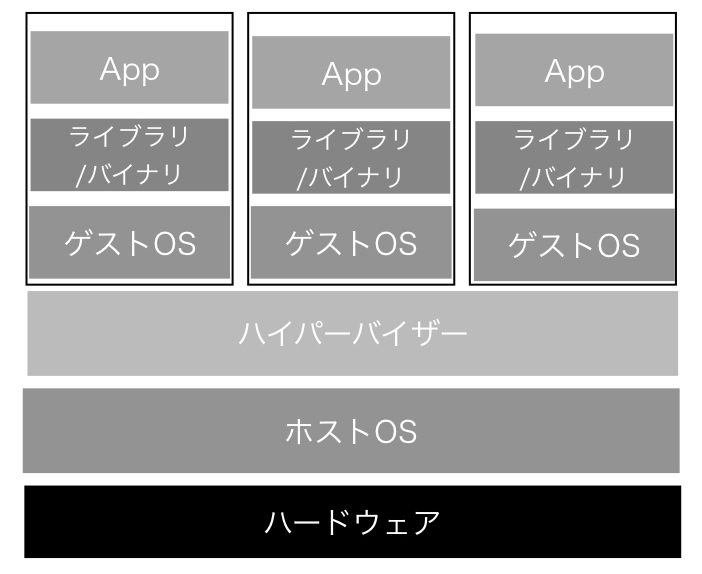
\includegraphics[width=80mm]{./assets/sample-chikuwa_ITasset/gray/host.jpeg}
    \caption{ホスト型ハイパーバイザ}
    \label{fig:hosthypervisor}
\end{figure}
\section{コンテナ型仮想化}
コンテナ型仮想化はハイパーバイザによる仮想化とは少し違う存在で, 単一のOS上に「コンテナ」と呼ばれる仮想的なユーザ空間を提供しています. ここ最近Dockerと呼ばれるコンテナランタイムの普及により注目される存在となってきました. またDocker以外にもLXC/LXDやHaconiwaといった様々なコンテナランタイムが登場しています. これらのコンテナランタイムは一見するとホスト型ハイパーバイザのようにOSの上でOSを簡単に起動しているように錯覚しがちですが, あくまでもコンテナではホストOSの一つの「プロセス」であり,リソースなどを制限したり切り分けていることで一つの小さな独立した環境を作っています. ここからはLinuxコンテナランタイムに焦点を絞り, Linuxのどのような機能を使ってコンテナというものを作り上げていくかを解説していきます.
\section{Linuxコンテナランタイムをつくり上げる技術}
\subsection{chroot}
chrootでは,図2.7のように現在のプロセスとその子プロセスのルートディレクトリを変更します. chroot後の環境から, 別のルートディレクトリや親のファイルシステムを見ることはできません. そのため, chroot監獄とも呼ばれます.しかしながら, chrootした環境内でchrootができる場合, この監獄はすぐに抜けることができてしまうため, 後述するnamespaceやcapabilitiesと併用して安全性を確保します.
\begin{figure}[htbp]
    \centering
    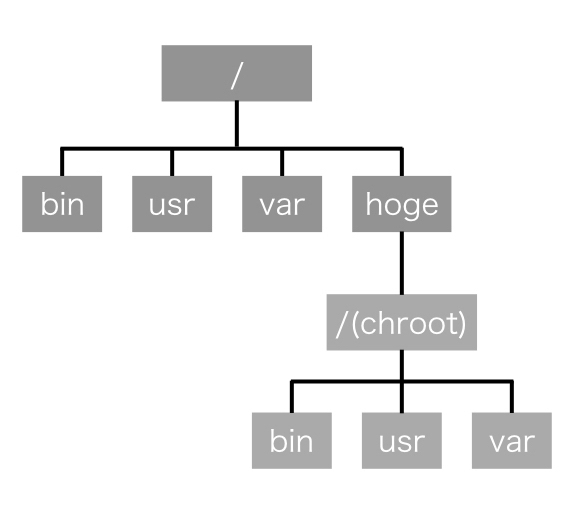
\includegraphics[width=80mm]{./assets/sample-chikuwa_ITasset/gray/chroot.jpeg}
    \caption{chroot}
    \label{fig:chroot}
\end{figure}

\subsection{cgroups}
cgroupsは, プロセスをグループ化してCPUやメモリなどのリソースをコントロールする仕組みです. cgroupsを使うことでCPUのコア数やリソースへのアクセスを再割り当てする一定間隔などを詳細に設定することはもちろん, プロセス数を制限してfork bomb対策をするなどの用途として使用します.
\subsection{Linux namespace}
Linux namespaceはOSのリソースの分離をおこなう仕組みです. Linuxの様々なリソースには「名前空間」と呼ばれるものが存在します. この名前空間を分けてあげることであたかもそのリソースしか存在しないように見せることでリソースを共存させることができます. 今回は4つの名前空間について解説します.
\subsubsection{IPC名前空間}
IPC名前空間はプロセス間通信のリソースであるSystem V IPCオブジェクトとPOSIXメッセージキュー(Linux2.6.30以降)を分離します. IPC名前空間で分離することによって名前空間が異なるプロセスが共有する共有メモリやセマフォにアクセスすることを防ぐことができます.
\subsubsection{Mount名前空間}
Mount名前空間は図2.8のようにファイルシステムのマウントポイントを分離することで異なる名前空間のファイルシステムにアクセスを分離することができます. 通常, 子プロセスは親プロセスと同じマウントポイントを認識します. しかし新しいMount名前空間の下では, 子プロセスは任意の変更を加えることができ,親プロセスやシステム全体のMount名前空間には影響を与えません. 例えば, 各コンテナごとにMount名前空間を分けて/var, /tmpを持たせることで独立したユーザ領域を見せることができます.
\begin{figure}[htbp]
    \centering
    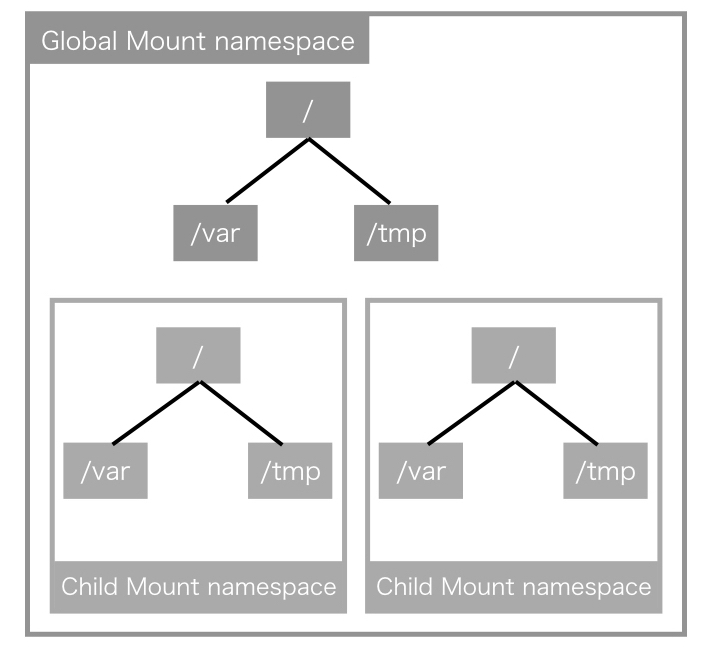
\includegraphics[width=50mm]{./assets/sample-chikuwa_ITasset/gray/mount.jpeg}
    \caption{Mount名前空間}
    \label{fig:mount}
\end{figure}

\subsubsection{PID名前空間}
PID名前空間では, 図2.9のようにプロセスID空間を分離します. 異なるPID名前空間では同じプロセスIDを持つことができ, 子名前空間内のプロセスは親のプロセスについて知ることができません. しかしながら, 親名前空間のプロセスは子名前空間のプロセスについて知ることができます. PID名前空間をコンテナごとに分離することで, コンテナ内のプロセス群を中断再開することやコンテナ内のプロセスのPIDを保持したままコンテナを別のホストに移したりするようなことが可能になります.
\begin{figure}[htbp]
    \centering
    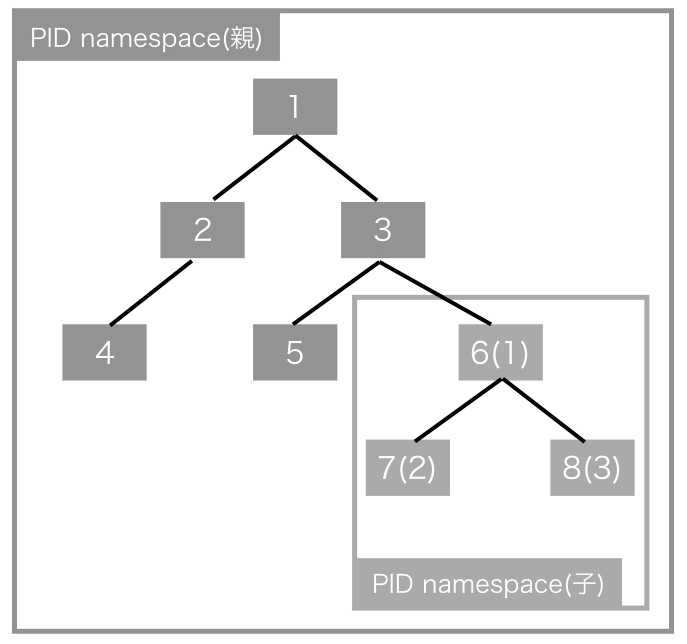
\includegraphics[width=50mm]{./assets/sample-chikuwa_ITasset/gray/pid.jpeg}
    \caption{PID名前空間}
    \label{fig:pid}
\end{figure}

\subsubsection{UTS名前空間}
UTS名前空間では,uname()というシステムコールで返されるホスト名とNISドメイン名を分離します. コンテナでUTS名前空間を分離することによって独自のホスト名とNISドメイン名を設定することができます.
\subsection{capabilities}
Linuxのプロセスには, 特権プロセスと非特権プロセスの2種類が存在します. 例えば, nginxなどのHTTPサーバが1024番ポート未満の特権ポートを使用する際などにプロセスに特権が必要となります. しかし, プロセスにすべての権限を与えてしまうとセキュリティ上あまり良いとは言えず, もっと細分化した権限を与えたい場合があります. そこでLinuxのcapabilitiesでは, 権限をCapabilityと呼ばれる細分化された単位でプロセスに与えることで特権を使用する頻度を下げることができます. capabilitiesは, カーネルのバージョンによって大きく異なりますが/usr/include/linux/capability.h内にある「CAP」からはじまるものがそのカーネルで使うことができるcapabilitiesです. 例えば, CAP\_NET\_BIND\_SERVICEはインターネットドメインの1024番未満の特権ポートをバインドできる権限です. そしてプロセスにはeffective・permitted・inheritableの3種類のケーパビリティ・セットと呼ばれるものがあり, 32ビットのビット列で持っているcapabilitiesを表現しています. effectiveは実際に使用することのできるケーパビリティ・セットで, permittedはプロセスが持つことを許可されているケーパビリティ・セット, inheritableはexecuveの前後で引き継がれるケーパビリティ・セットです.
\section{おわりに}
クラウドやDockerの普及等によってエンジニアにとって仮想化技術というものは当たり前にあるような存在にはなってきましたが, 概念的にも技術的に難しく中々理解したり実装することは難しいです.しかし, ぜひこの機会に普段使っているよう仮想化技術がどのようにして出来上がっているのかを見なおしてみると様々なことを知ることができて楽しいはずです.例えば簡単なLinuxコンテナならシェルだけでも出来てしまいますし, 興味があるならぜひやってみると楽しいと思います.


\chapterauthor{はいばら}
\chapter{LOCAL学生部 活動報告}
\section{はじめに}


\subsection{SecHack365(1期)}
\begin{description}
\item[参加部員] さわだ
\end{description}

SecHack365は国立研究開発法人情報通信研究機構(NICT)が主催する,若手セキュリティイノベーターを育成する長期ハッカソンです.
その初年度にさわださんが参加しました.\mbox{}\\

\begin{description}
\item[さわださんはSecHack参加者の海外派遣として,SXSWにも参加したそうです!]\mbox{}\\
SecHack365 0xFF SXSW Part.1\mbox{}\\
\url{https://takuzoo3868.hatenablog.com/entry/sechack365_0xff_part1}
\end{description}

\subsection{SecHack365(2期)}
\begin{description}
\item[参加部員] あるねこ・壱・もぐら
\end{description}

同じくSecHackの第2期です.あるねこさん・壱さん・もぐらさんが参加しました.\mbox{}\\

\begin{description}
\item[SecHack沖縄回の帰路,飛行機の中で書いたという,壱さんのブログ.]\mbox{}\\
SecHack365な1年と次の参加者に向けて\mbox{}\\
\url{https://ich1-one.hatenablog.com/entry/2019/04/04/234234}
\end{description}

\begin{description}
\item[あるねこさんの作品は優秀作品に選ばれたそうです!]\mbox{}\\
あるねこさん的SecHack365参加録\mbox{}\\
\url{https://www.aruneko.net/post/sechack_2018/}
\end{description}


\subsection{Web×IoT メイカーズチャレンジ 2018-19 in 札幌}
\begin{description}
\item[参加部員] はいばら
\end{description}

Web×IoT メイカーズチャレンジはIoTシステム開発のスキルアップを目的としたハンズオン\and ハッカソンです.\mbox{}\\

\begin{description}
\item[札幌でのハッカソンで技術賞をいただきました.]\mbox{}\\
Web×IoT メイカーズチャレンジ 2018-19 in 札幌 に行ってきました\mbox{}\\
\url{https://haibara-works.hatenablog.com/entry/2018/11/29/000835}
\end{description}


\subsection{セキュリティ・ミニキャンプ in 北海道}
\begin{description}
\item[参加部員] あるねこ・壱・がっちゃん・はいばら・すとんりばー
\end{description}

セキュリティ・ミニキャンプ(地方大会)は,若年層を対象とした情報セキュリティ人材の育成のための講習会です\mbox{}\\

\begin{description}
\item[セキュリティ・ミニキャンプ in 北海道 2018]\mbox{}\\
\url{https://www.security-camp.or.jp/minicamp/hokkaido2018.html}
\end{description}\mbox{}\\

\begin{quotation}
IoTデバイスのセキュリティやC言語の不適切なコーディングによって産まれる脆弱性,USBデバイスの開発方法を学びました.
また,北海道警察の方から『セキュリティ技術と倫理』についてお話をいただきました.(はいばら)
\end{quotation}

\subsection{HOKKAIDO学生アプリコンテスト2019}
HOKKAIDO学生アプリコンテストは"モバイルアプリケーションの企画力、デザイン力、プログラム力を有する学生を表彰することにより、学生のモバイル分野に対する関心を高め、次代を担う高度なモバイルIT人材の発掘・育成に寄与することを目的"としたコンテストです.\mbox{}\\

\begin{quotation}
アプリコンテストには2回目の参加で、企業賞をいただけて嬉しかったです!次のコンテストに繋げられるようにこれからも頑張りたいです!(ことみん)
\end{quotation}

\subsection{YAPC}
\begin{description}
\item[参加部員] 那由多・ことみん
\end{description}
YAPC(Yet Another Perl Conference)は"Perlを軸としたITに関わる全ての人のためのカンファレンス"です.\mbox{}\\

\begin{description}
\item[那由多のブログ.スクラム開発に興味をもったようです.]\mbox{}\\
いってきましたYAPC::Tokyo 2019\mbox{}\\
\url{https://nayuta-1999.hatenablog.com/entry/2019/01/30/145145}
\end{description}

\begin{description}
\item[ことみんのブログ.前夜祭のLTソンから参加したそうです!]\mbox{}\\
ブログを書くまでがYAPC::Tokyoです。\mbox{}\\
\url{https://kotomi1338.hatenablog.com/entry/2019/01/29/235640}
\end{description}

\subsection{OSC Hokkaido}
オープンソースの文化祭 OSC Hokkaido 2018では学生部でブース展示をしました.また,開催レポートの執筆も担当しました.\mbox{}\\
\begin{description}
\item[昨年より多くの参加者で賑わった OSC2018 Hokkaido]\mbox{}\\
\url{https://www.ospn.jp/press/20180717osc2018-hokkaido-report.html}
\end{description}

\subsection{LOCAL学生部総大会}
LOCAL学生部総大会は,学生部の年一度のオフラインイベントです.2018年度の開催では,さくらインターネットさんの石狩DCで合宿するという,スペシャルな回になりました!\mbox{}\\

\begin{description}
\item[LOCAL学生部のブログ]\mbox{}\\
第10回 LOCAL学生部総大会 開催レポート\mbox{}\\
\url{http://students.local.or.jp/blog/entry/2018/08/23}
\end{description}

\begin{description}
\item[けんつさんのブログ]\mbox{}\\
第10回LOCAL学生部総大会をやってきました\mbox{}\\
\url{http://rabbitfoot141.hatenablog.com/entry/2018/10/06/233550}
\end{description}

\begin{description}
\item[ともかさんのブログ]\mbox{}\\
LOCAL学生部のイベントに初参加してきましたよっ!\mbox{}\\
\url{https://mokomoka.hateblo.jp/entry/localst18}
\end{description}

\begin{description}
\item[はいばらのブログ]\mbox{}\\
行ってきました第10回LOCAL学生部総大会\mbox{}\\
\url{https://haibara-works.hatenablog.com/entry/2018/10/08/113256}
\end{description}

\begin{description}
\item[しかさんのブログ]\mbox{}\\
楽しかった総大会\mbox{}\\
\url{https://sika0115.hatenablog.com/entry/2018/10/07/191213?_ga=2.55916011.1590347690.1538897406-1485988726.1512910189}
\end{description}

\begin{description}
\item[ことみんのブログ]\mbox{}\\
LOCAL学生部の楽しい集まりがありました。\mbox{}\\
\url{https://kotomi1338.hatenablog.com/entry/2018/09/30/225711}
\end{description}

\subsection{技術書典4}
技術書典4にて,学生部の同人誌 第一弾『情報ボーイズの寄稿ノート』を頒布しました.
COMIC ZINにて委託販売も行っておりますので,ご興味のある方は是非お求めください!\url{https://shop.comiczin.jp/products/detail.php?product_id=36441}\mbox{}\\

以下,技術書典4 サークルページから引用.(\url{https://techbookfest.org/event/tbf04/circle/14720002}})
\begin{quote}
\begin{description}
\item[概要]\mbox{}\\ 
北海道の学生が集結して作成したオムニバス形式の同人誌.みんな"得意なことは違う"ので,バラエティ豊かな内容になりました.ぜひ手に取ってみてください!

\item[目次]\mbox{}\\ 
\begin{description}
\item[\LaTeX の乱数生成アルゴリズムを調べる]\mbox{}\\ 
\LaTeX 標準の乱数パッケージはFortran由来だった?そんな乱数パッケージの詳細について徹底的に調べてみました.
\item[超入門 仮想化技術]\mbox{}\\ 
仮想化って色々ありすぎてわからない.そんなあなたに仮想化技術の基礎から解説します.
\item[LEDで発電しよう!!!]\mbox{}\\ 
LEDは電力を与えると光るので,逆に光を与えると発電できるのでは.そんな現象を実験で確かめました.
\item[入門Linux Kernel]\mbox{}\\ 
Linux Kernelモジュールの作成方法をサンプルコード付きでわかりやすく解説します.
\item[自作エディタ入門編]\mbox{}\\ 
宗教戦争の果てに,自分だけのエディタを作るお話です.
\item[世界と孤独の説法(エピローグ)]\mbox{}\\ 
PDFで遊べる新感覚のゲーム.紙バージョンでは掲載しきれなかったのでPDF版でお楽しみください.
\item[関数型Python入門]\mbox{}\\ 
PythonでMonadを作りながら,型ヒンティング機能で遊び尽くします.型ヒントを使ってみたいあなたにもオススメ!
\end{description}
\end{description}

\end{quote}

  
\newpage
\myimpression[%
name=LOCAL Students\\情報ボーイズの寄稿ノート 2.0, %
author=はいばら, \and %
ちくうぇいと, %
date=2020年5月3日, %
publisher=LOCAL学生部, %
print=有限会社ねこのしっぽ %
]%
\end{document}
